% Companion Pandoc template: preserve the original CPB Beamer preamble and layout.
\documentclass[aspectratio=169,11pt,handout,xcolor=dvipsnames]{beamer}

\usepackage[utf8]{inputenc}
\usepackage[T1]{fontenc}
\graphicspath{{../}}
\makeatletter
\def\input@path{{../}}
\makeatother
\usepackage{cpb-beamer} % Reuse the original CPB style from the parent folder.
\usepackage[dutch,english]{babel}  % Gebruik [english, dutch]{babel} voor nederlandse datumnotatie
\usepackage{booktabs}
\usepackage{colortbl}
\usepackage{array}
\newcommand{\mypos}[2]{\tikz[remember picture]{\node[inner sep=0pt, anchor=base](#2){#1};}}
\newcommand{\myund}{}
\usepackage{pgfplots}
\pgfplotsset{compat=1.18}
\usepackage{adjustbox}  % voor clippen van achtergrondafbeelding
\usepackage{setspace}
\usepackage{soul}
\usepackage{natbib} % voor using bibliographystyle amcg
\usepackage{bm}
\usepackage{amsmath,amsfonts,eqnarray}
\usepackage{amssymb,dsfont,bbold}
\usepackage{changepage}
\usepackage{nicefrac}
\usepackage{multirow}
\usepackage{subcaption}


\title[Two columns]{Two-column slides}
\author{CPB}
\disclaimer{}
\eventtype{Event type}
\date{\today}
\cpbfooter{CPB}
\cpbtitelafbeelding{} % Titel figuur

\providecommand{\tightlist}{}
\begin{document}
\begin{frame}{My slide}
\label{my-slide}
\begin{columns}[T,onlytextwidth]
\begin{column}{0.48\textwidth}
\begin{itemize}
\tightlist
\item
  First point
\item
  Second point
  \begin{itemize}
  \tightlist
  \item
    A nested point
  \end{itemize}
\end{itemize}

\end{column}
\hfill
\begin{column}{0.48\textwidth}

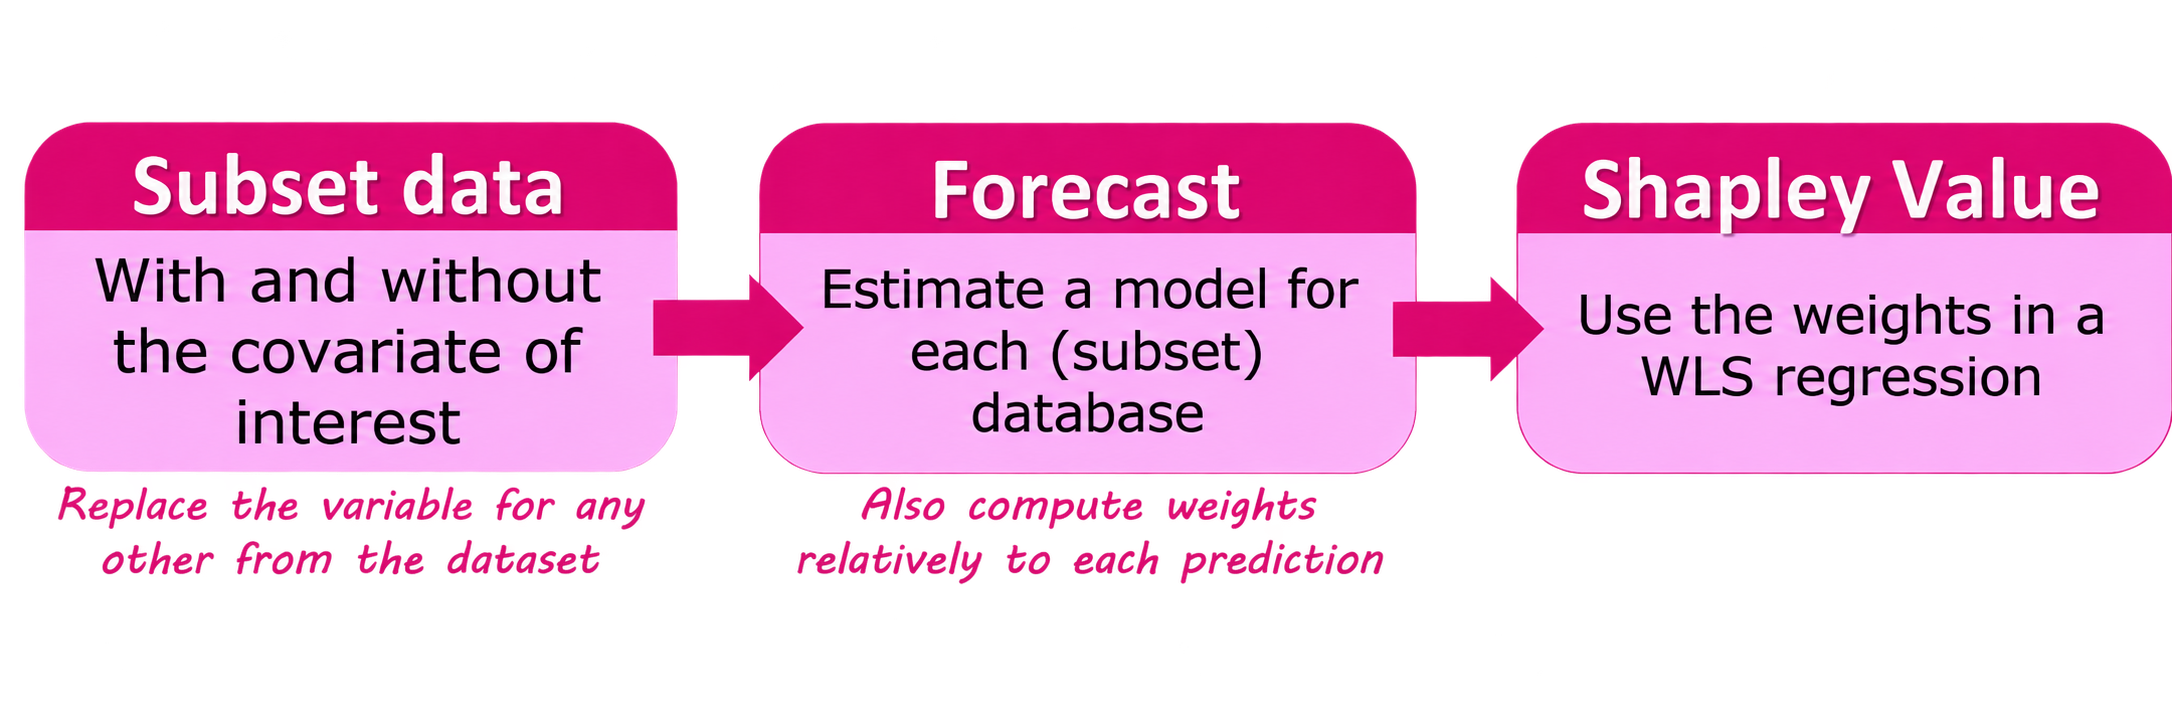
\includegraphics[width=1\linewidth,height=\textheight,keepaspectratio,alt={Example figure}]{../Figures/SHAP2.png}

\end{column}
\end{columns}
\end{frame}

\begin{frame}[fragile]{Another slide}
\label{another-slide}
\begin{itemize}
\tightlist
\item
  Back to a normal full-width slide.
\item
  Start another two-column slide by adding \verb|{.split}| to its heading.
\end{itemize}
\end{frame}

\begin{frame}{A block}
\label{a-block}
\begin{block}{Task}
\begin{itemize}
\tightlist
\item
  First point
\item
  Second point with \textbf{bold text}
\end{itemize}
\end{block}

This text is outside the block.
\end{frame}

\begin{frame}{A diagram}
\label{a-diagram}
\begin{figure}
\centering
\resizebox{0.8\linewidth}{!}{%
\cpbdiagram{blue}{3}{%
\cpbdiagramitem{Box 1}{Text 1}{Caption 1}
\cpbdiagramitem{Box 2}{Text 2}{Caption 2}
\cpbdiagramitem{Box 3}{Text 3}{}
}}
\caption{Example of a blue diagram}
\end{figure}
\end{frame}
\end{document}
